\chapter{Hardware}

Modern computers are a complex group of devices working together
to perform a common task (or tasks). A user will interact with a
computer through a variety of input and output devices (e.g.
keyboards, mice, speakers, microphone, and monitors). A user's
input will be processed, some computations will be performed, and
then the resulting output will be displayed to the user. When most
of us thinking about computers, we often think of a desktop or laptop
computer, that come equipped with a keyboard, mouse, and monitor;
however, many things we interact with daily are computerized,
including cell phones, cars, traffic lights, smart watches,
televisions, and manufacturing lines. Today each of these items
have sensors to perceive the real world, use an embedded computing
device to understand the sensory input, and use a combination of
display and mechanical devices to interact with the real world.

\begin{example}
For intersections across busy roadways, some traffic lights are
computerized to optimize road traffic. These lights will stay
green along the busier of the two roads, and use cameras or
pressure sensors to detect the presence of cars along the less
busy of the two roads, thus switching to allowing the cars on
the less busy road to cross when it arrives. Overall, providing
a less congested intersection by relying on an embedded computer.
\end{example}

Today we will introduce three fundamental parts of computer systems:
input and output devices, memory, and the central processing unit (CPU).
These components work together to perform the basic building blocks of
input processing, storage, control, and output. Understanding how the
three parts work together will allow us to create powerful information
processing tools. We will introduce each of these parts in turn.
In figure~\ref{fig:hardware:overview}, we see how these parts come
together to form a computer system (similar to the ones you'll use
to program in this course).

\begin{figure}
	\centering
	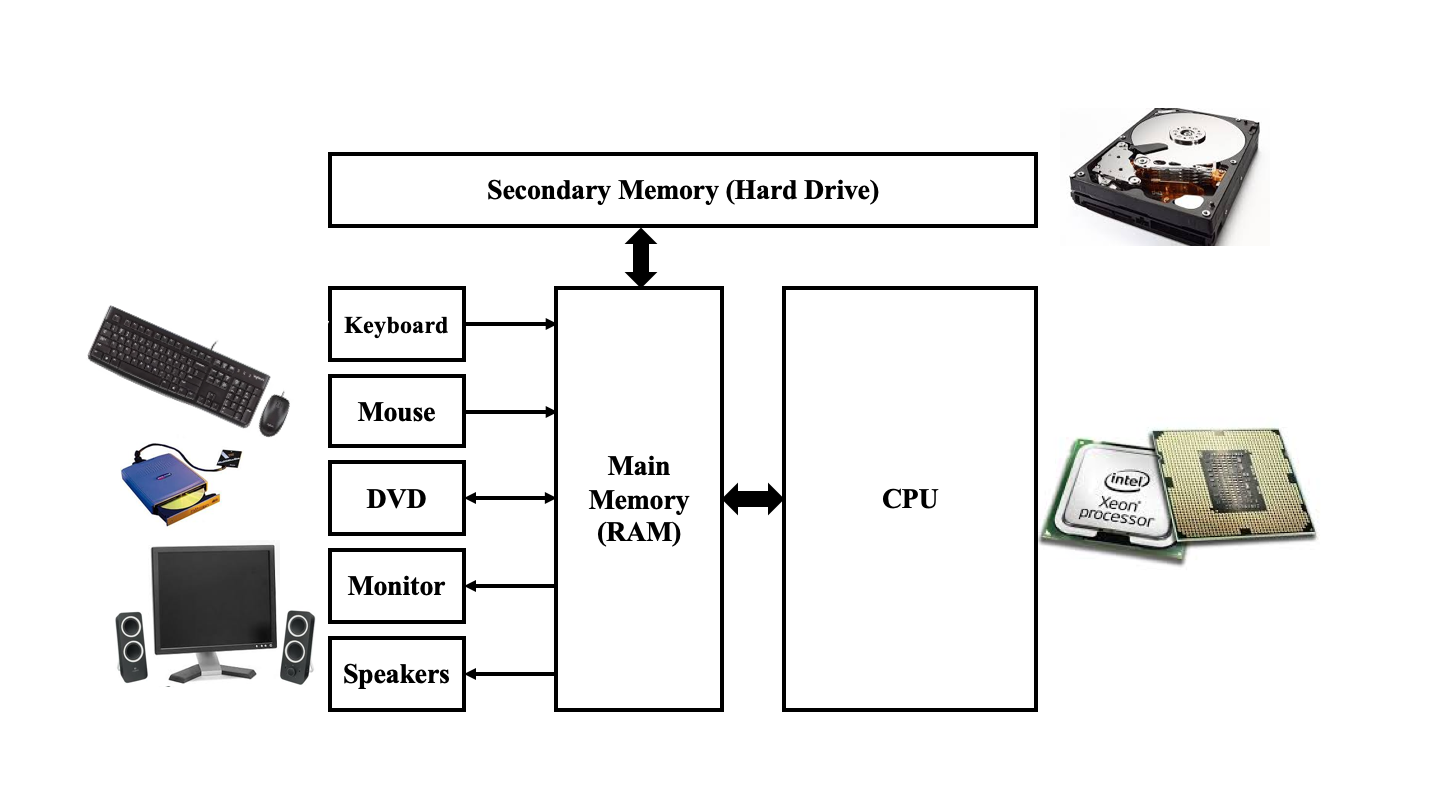
\includegraphics[width=0.85\textwidth]{images/cs_intro_hardware_overview.png}
	\caption{Interconnected parts of a computer system (keyboard, mouse,
                 monitor, DVD player / burner, speaker, hard drive, CPU).}
	\label{fig:hardware:overview}
\end{figure}

\section{Input and Output Devices}

We will begin by discussing input and output devices. These devices
allow the computer to interact with users and the world directly. Without
these devices, a computer system would be very boring, always performing
the same computation each time it's used. Even if it did compute a different
value we would be unable to examine the value. A computer needs to be
able to accept input and allow output. The first computers would occupy
a large room in an office building and connect to a terminal
(a keyboard and a text screen) in another room for users to interact
with. Thanks to Moore's Law, computers many orders of magnituted more
powerful can fit in the palm of your hand. Likewise, the variety of input
and output devices has multipled. We still have the keyboard and monitor,
we've added the mouse for interacting with graphical displays. Today's
phones are more computer than phone, coming equipped with: speakers,
microphones, touch screens, cameras, fingerprint scanners, radio transmitters,
and much more. Computers even come embedded in other devices like cars,
traffic lights, X-ray machines, and thermostats to both control and
monitor the devices. As shown in Figure~\ref{fig:hardware:overview},
these devices connect to the rest of the computer through the computer's memory.
This kind of input and output is called memory mapped I/O (input and output).
Creaters of input (or output) devices are assigned a section of the
computer's memory to write (read resp.) data. The computer will then read
(write resp.) data to those locations to communicate with the given device.
The creaters of these devices, agree upon a known format to read and write data.

\begin{example}
You can think of this communication between devices and computer similar to
leaving messages for a friend in a locker. Only you and your friend have
access to this locker, which only holds space for one message. The format
you agree upon is which language you'll use to speak (e.g. English) and any
special keywords or phrases. You might agree with your friend, that if either
of you write a message saying ``The morning is upon us'' that the other will
wait until ``The night has come'' before leaving any new messages.
\end {example}

The format that devices and computers communicate in are generally very simple
and structured to permit fast and easily understandable communication for
computers and devices.

\begin{example}
A monitor is a graphical display for computers. Let's consider a monitor
connected to a computer that only displays in black and white images
that are 20 x 20 pixels large. The monitor and keyboard agree upon using
the following format to communicate. The format is black and white images
that are 20 x 20 pixels large. Each pixel's value is represented at 0 for
black and 1 for white. Then an image is represented as a 400 = (20 x 20) long
sequence of pixel values. The sequence is ordered left to right, top to bottom.
Now that both the monitor and computer agree upon the communication format, the
computer can write images to the section of memory dedicated to the monitor
and the monitor will read the image and display the image on it's screen.

\emph{Note: while this is a simplified example, this is similar to how modern
graphical displays communicate with computers}.
\end{example}

\section{Memory}

Another fundamental part of a computer, is the memory. There are two major types
of memory, Main Memory (RAM), and Secondary Memory (e.g. hard disks, solid-state
drves, tape drives, etc.) Main memory is volatile, meaning that the contents
of the memory is not preserved when a computer is turned off and back on. On the
other hand Secondary Memory, is meant to be persistent (the opposite of volatile).
Main Memory can be thought of as the ``scratch paper'' the computer uses for
computations. Computers will also use Main Memory as a conduit for communicating
between the CPU and all other parts of the computer. In most modern computers,
programs are treated as data. That is the individual instructions that combine
to form a program are stored in memory just as data is. It is the job of the
computer to properly understand if a segment of memory is data or a program.
The computer is able to fetch data from Secondary Memory to Main Memory or
persist data in Main Memory to Secondary Memory when needed.

\section {Central Processing Unit}

The final part of a computer we will introduce today is the central processing
unit (CPU) --- processor, main processor, etc. The CPU is the physical
circuitry of a computer that performs instructions. The CPU is responsible for
fetching, decoding, and executing all instructions. These instructions form the
basic bulding blocks of all programs. These instructions vary between different
brands of CPUs but in general they will include arithmetric, control, input, and
output functionalities.

\begin{example}
\begin{verbatim}
load R1 16    -- Load value at memory location 16 into register 1
load R2 20    -- load value at memory location 20 into register 2
add  R1 R2 R1 -- add the value in register 1 to the value in register 2
                 and store in register 1
store R1 16   -- store the value in register 1 to memory location 16
\end{verbatim}
\end{example}


The CPU is in charge of fetching, decoding, and
executing all instructions. The basic building blocks of these instructions include arithmetic, logic,
control, input, and output. The set of basic instructions available to the CPU effects, what the computer
system can do (and how efficiently). Some CPU's are designed to handle a relatively small number of
instructions (integer addition, multiplication, division, conditional branching, store to memory, load
to memory). While others CPU's are designed to handle a large number of instructions (e.g. swap content
of memory locations, increment and store, etc. in addition to the simpler instructions).

While these instructions can be quite simple, we build up complex behaviours by combining these actions
into programs. When reasoning about how our programs will work, we should be aware of the limitations
imposed by the hardware we use. In mathematics, we often consider things in a very abstract way. In models
of computer systems, we often use unbounded arithmetic and allow a computer to have infinite memory; however,
in practice we need to run programs on processors with bounded computational and memory capabilities. In most
systems we encounter today, the CPU allows for 32 or 64 bit computations or memory read and writes in a single
instruction. Because reading and writing to memory takes a long time (in comparison to arithemetic and logic
instructions), almost all CPUs include a very small number of memory blocks on the physical CPU to store
intermediate results of instructions, called registers. In modern CPUs this is further increased by allowing
even more levels of memory, called caches (Level 1, Level 2, and Level 3), that trade off between speed of access
and the size of the memory. We won't go in depth on how these work, but briefly mention them to help you
understand how modern computer systems work to acheive greater efficiency.
